\documentclass[a4j]{jarticle}

\usepackage[dvipdfmx]{graphicx}
\usepackage{url}
\usepackage{here}
%\usepackage{listings}
\usepackage{amsmath,amssymb}
\usepackage[dvipdfmx]{color}

\setlength{\headsep}{-5mm}
\setlength{\oddsidemargin}{0mm}
\setlength{\textwidth}{165mm}
\setlength{\textheight}{230mm}
\setlength{\footskip}{20mm}

\title{
\vspace{30mm}
{\bf 子育て支援システム}
\\
\vspace{5mm}
{\bf 外部設計書v2\\
}
\vspace{120mm}
}

\author{
\vspace{5mm}
チーム名 007\\
\vspace{5mm}
}


\begin{document}
\maketitle
\tableofcontents
\newpage

\section{はじめに}
本書では弊社がシステム提案書で提案した子育て支援システムの詳細を示しています。

まず、本システムの概要及びシステムを構成するサブシステムについて示します。
次に本システムのユーザインタフェースについて示し、最後に本システムを構築するデータテーブル設計に
ついて示します。

\section{システム概要}
本システムは機能として成長記録機能、ゲーム機能、子育て窓口機能、設定機能の4つを実装します。この章では、各機能の説明及び各機能を構成するサブシステムを示します。サブシステムの詳細は第3章にて説明します。

\subsection{成長記録機能}
成長記録機能では、日々の子供の成長を記録できる機能を提供します。成長記録は日付ごとに分けて記録され、いつでも見返すことができます。外部アプリ(Twitter)で記録を共有することもできます。
\subsubsection*{構成サブシステム}
\noindent カメラ撮影サブシステム、コメント記録サブシステム、ゲーム結果取得サブシステム、カレンダーサブシステム、共有サブシステム

\subsection{ゲーム機能}
ゲーム機能では、2〜5歳を対象とした簡単な知育ゲームを提供します。おえかきとおつかいのゲームがあり、お絵描きではゲームの記録を成長記録機能に保存することが可能です。
\subsubsection*{構築サブシステム}
\noindent ペイントサブシステム、おつかいサブシステム、ゲーム記録保存サブシステム、ゲーム追加サブシステム

\subsection{子育て窓口機能}
子育て窓口機能では、子育てに関する質問を投稿・回答することができる機能を提供します。質問の検索も可能です。
\subsubsection*{構築サブシステム}
\noindent 検索サブシステム、並び替えサブシステム、投稿サブシステム、回答サブシステム

\subsection{設定機能}
本システムを初めて利用する場合は、本システムの機能の1つである子育て窓口機能を利用するために初期設定としてアカウント登録を行う必要があります。他にも、子供がゲーム機能から別の機能に遷移してトラブルが起きることを防止するために、ゲーム画面からメニュー画面に戻るためのパスワード設定を行うことを推奨します。設定機能では、アカウント登録と緊急時の問い合わせ(メール)、アカウント情報の変更と削除、ゲームのパスワード設定を行うことができます。
\subsubsection*{構成サブシステム}
\noindent アカウント登録サブシステム、メール問い合わせサブシステム、アカウント情報サブシステム、ゲームのパスワード設定サブシステム



%サブシステム%
\newpage
\section{サブシステム概要}
第2章で述べている4つの機能を構成しているサブシステムについて説明します。

\subsection{成長記録機能}
\subsubsection*{カメラ撮影サブシステム}
利用端末に搭載されているカメラをシステム内から起動し、写真を撮影することができます。
\subsubsection*{コメント記録サブシステム}
保存されている成長記録(写真、ゲームの結果)に対してコメントを記述することができます。成長記録を見ながらコメントを読み返すことにより、過去の思い出が振り返りやすくなります。
\subsubsection*{ゲーム結果取得サブシステム}
ゲーム機能で子供が遊んだ結果を成長記録として保存することができます。
\subsubsection*{カレンダーサブシステム}
成長記録を日付ごとに分けるサブシステムです。本システムの利用者は、画面に表示される写真を選択することによって、保存された成長記録を確認することができます。
\subsubsection*{共有サブシステム}
成長記録を他のSNSアプリケーションで共有することができます。

\subsection{ゲーム機能}
\subsubsection*{ペイントサブシステム}
お絵描きのゲームを提供します。お手本を見ながら同じものを描く機能と自由に描く機能を設けます。
\subsubsection*{おつかいサブシステム}
おつかいのゲームを提供します。特定の料理の材料を買うことで料理が完成するという内容です。
\subsubsection*{ゲーム記録保存サブシステム}
お絵描きの記録を保存するサブシステムです。保存されることにより成長記録機能での記録の閲覧が可能です。
\subsubsection*{ゲーム追加サブシステム}
新しくゲームの追加を行います。またゲームの削除や変更も行います。今後この機能を利用してゲームの種類の増加を図ります。

\subsection{子育て窓口機能}
\subsubsection*{検索サブシステム}
質問の検索を行うサブシステムです。 質問したい内容・ワードを入力することで質問の内容・ワードに合致したものが表示されます。
\subsubsection*{並び替えサブシステム}
投稿された質問を並び替えるサブシステムです。
\subsubsection*{投稿サブシステム}
質問を投稿するサブシステムです。
\subsubsection*{回答サブシステム}
質問に回答を行うサブシステムです。

\subsection{設定機能}
\subsubsection*{アカウント登録サブシステム}
システムを初めて利用する際にアカウント登録を行います。登録する情報は、名前(ニックネーム可)と住んでいる都道府県です。
\subsubsection*{メール問い合わせサブシステム}
本システムについてトラブルや質問など何か問い合わせをしたいときに、メールを管理者に送ることができます。
\subsubsection*{アカウント情報サブシステム}
アカウント情報の変更及びアカウントの削除を行うことができます。しかし、子育て窓口機能で投稿した内容などは削除されません。
\subsubsection*{ゲームのパスワード設定サブシステム}
ゲーム画面からメニュー画面に戻るためのパスワード設定を行うことができます。

%%ユーザインタフェース(UI)%%
\newpage
\section{ユーザインタフェース}
本章では、システムを構成するユーザインタフェースについて示します。

%初期画面%
\subsection{画面詳細}
本システムが提供するアプリケーションの画面遷移及び画面の詳細について説明します。
\subsubsection{初期設定画面}
図\ref{honjo_setup}に、アプリを初めて起動した際に表示される初期設定画面を示します。
この画面はユーザに『名前(ニックネーム)の入力』・『居住地域の選択』を行ってもらうために表示されます。
入力が完了しないと次の画面に遷移することはできません。

また、再インストールをした場合であってもこの画面が表示され、再度設定(ユーザの新規作成)を行う必要があります。

図\ref{honjo_setup}に示す番号と対応させる形式で、以下にその役割を示します。

\begin{figure}[H]
    \begin{center}
    \resizebox{8cm}{!}{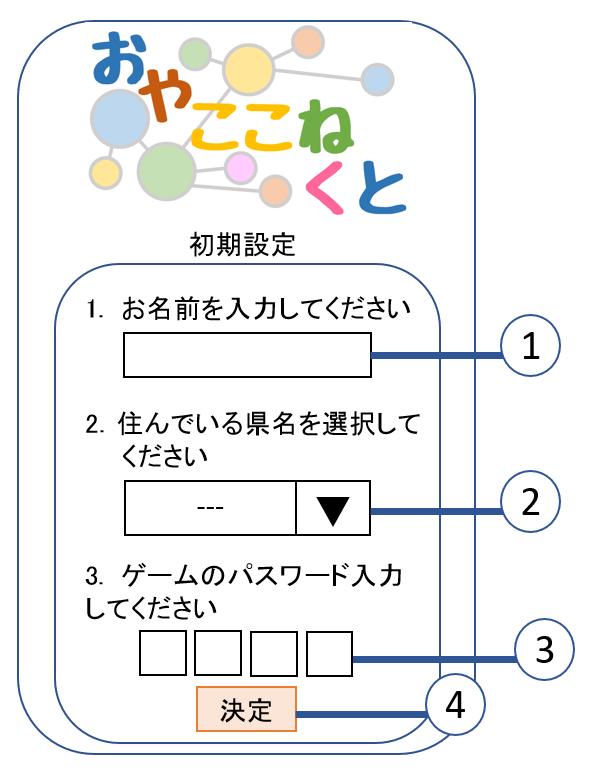
\includegraphics {honjo_FirstSetting.png}}
    \caption {初期設定画面のイメージ}
    \label{honjo_setup}
    \end{center}
\end{figure}

\begin{enumerate}
  \renewcommand{\labelenumi}{\textcircled{\scriptsize \theenumi}}
  \item 名前(ニックネーム)の入力欄\\
        ユーザがアプリ内で使用したい名前を入力します。矩形領域をタップするとキーボードが開き、入力することが可能になります。
  \item 居住地域の選択欄\\
        ユーザの住んでいる地域を選択します。矩形領域をタップするとドロップダウンリストが開き、その中から住んでいる都道府県を選択します。
  \item ゲームのパスワードの入力欄\\
        ゲーム画面からメニュー画面に戻るためのパスワードを設定します。入力できるのは4桁の数字のみです。ここで設定したパスワードは後からでも変更することができます。
  \item 完了ボタン\\
        入力が完了したら押すボタンです。入力が正しくされている場合にのみメニュー画面(図\ref{honjo_main})へ遷移することができます。
\end{enumerate}


\subsubsection{メインメニュー画面}
図\ref{honjo_main}に、メインメニュー画面を示します。これは、アプリの初期設定を完了している場合に、最初に表示されます。
この画面は本アプリの持つ機能に遷移するために使用されます。

図\ref{honjo_main}に示す番号と対応させる形式で、以下にその役割を示します。

\begin{figure}[H]
    \begin{center}
    \resizebox{8cm}{!}{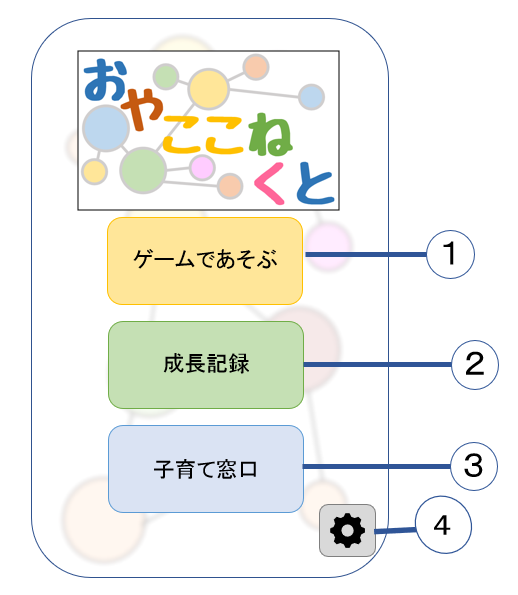
\includegraphics {honjo_main.png}}
    \caption {メインメニュー画面のイメージ}
    \label{honjo_main}
    \end{center}
\end{figure}

\begin{enumerate}
  \renewcommand{\labelenumi}{\textcircled{\scriptsize \theenumi}}
  \item ゲーム画面選択ボタン\\
        ゲーム機能を使用したい場合に押すボタンです。タップするとゲーム選択画面(図\ref{game})へ遷移します。
  \item 成長記録画面遷移ボタン\\
        成長記録機能を使用したい場合に押すボタンです。タップすると成長記録画面(図\ref{Grow})へ遷移します。
  \item 子育て窓口画面遷移ボタン\\
        子育て窓口機能を使用したい場合に押すボタンです。タップすると子育て窓口画面(図\ref{honjo_CR_Window})へ遷移します。
  \item 設定画面遷移ボタン\\
        アプリの設定を変更したい場合に押すボタンです。タップすると設定画面(図\ref{configuration})へ遷移します。
\end{enumerate}

%ゲーム%
\subsection{ゲーム選択画面}
図\ref{game}にゲームの選択画面を示します。\\
お絵描きとおつかいのゲームを提供します。

\begin{figure}[H]
    \begin{center}
    \resizebox{8cm}{!}{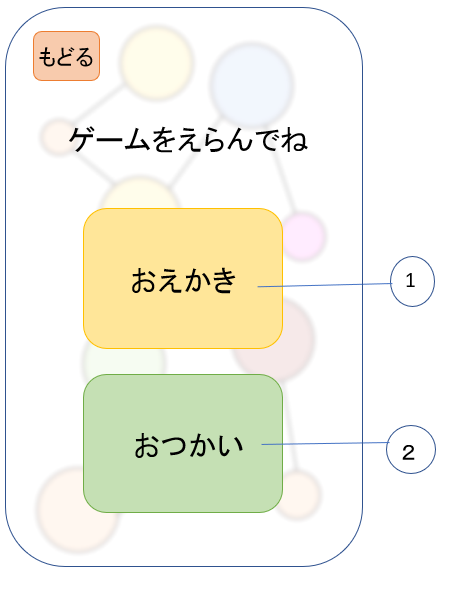
\includegraphics {game.png}}
    \caption {ゲーム選択画面のイメージ}
    \label{game}
    \end{center}
\end{figure}

\begin{enumerate}
  \renewcommand{\labelenumi}{\textcircled{\scriptsize \theenumi}}
\item もどるボタン\\
  もどるボタンをタップすることでパスワード画面(図\ref{password})に遷移します。
\item おえかき\\
  おえかきの矩形領域をタップするとお絵描きの詳細画面(図\ref{oekaki})へ遷移します。
\item おつかい\\
  おつかいの矩形領域をタップするとおつかいのゲーム画面(図\ref{otukai1})へ遷移します。
\end{enumerate}

\newpage
\subsubsection{パスワード画面}
図\ref{password}にパスワード画面を示します。\\

\begin{figure}[H]
    \begin{center}
    \resizebox{8cm}{!}{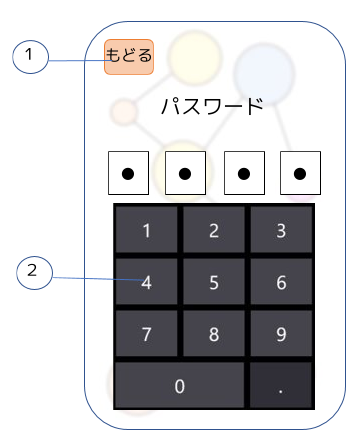
\includegraphics {password.png}}
    \caption {パスワード画面のイメージ}
    \label{password}
    \end{center}
\end{figure}

\begin{enumerate}
  \renewcommand{\labelenumi}{\textcircled{\scriptsize \theenumi}}
\item もどるボタン\\
  もどるボタンをタップすることでゲーム選択画面(図\ref{game})に遷移します。
\item キーボード\\
  キーボードの数字をタップしパスワードを打つことでメインメニュー画面(図\ref{honjo_main})に遷移します
\end{enumerate}

\newpage
\subsubsection{おえかきゲーム画面}
図\ref{oekaki}におえかきの詳細画面を示します。\\
画面上のボタンをタップすることでおえかきのモードを選択することができます。\\

\begin{figure}[H]
    \begin{center}
    \resizebox{8cm}{!}{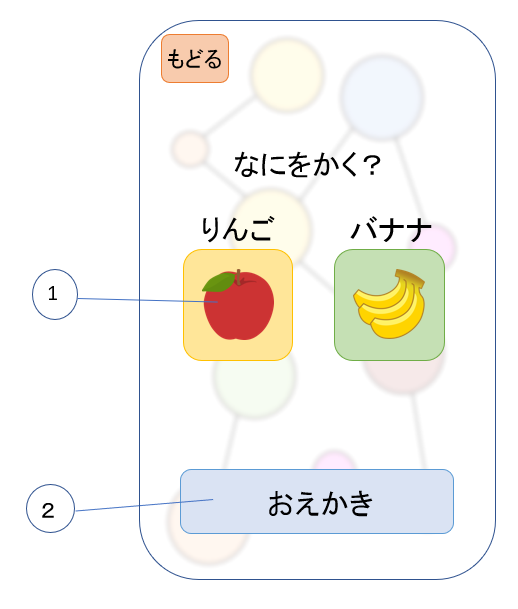
\includegraphics {oekaki.png}}
    \caption {おえかきゲーム画面のイメージ}
    \label{oekaki}
    \end{center}
\end{figure}

\begin{enumerate}
  \renewcommand{\labelenumi}{\textcircled{\scriptsize \theenumi}}
\item もどるボタン\\
  もどるボタンをタップするとゲーム選択画面(図\ref{game})に遷移します。
\item イラストボタン\\
  イラストのボタンをタップすることでイラストおえかき画面(図\ref{illustration})に遷移し、タップしたイラストを閲覧しながらのおえかきができます。
\item おえかきボタン\\
  おえかきのボタンをタップすることでおえかきのゲーム画面(図\ref{oekaki2})に遷移し、自由におえかきができます。
\end{enumerate}

\newpage
\subsubsection{イラストおえかき画面}
図\ref{illustration}はイラストおえかき画面を示します。\\

\begin{figure}[H]
  \begin{minipage}{0.5\hsize}
    \begin{center}
    \resizebox{8cm}{!}{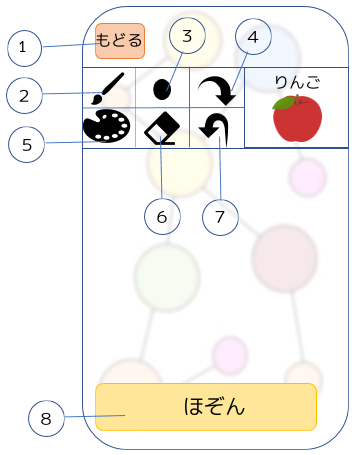
\includegraphics {illustration.png}}
    \caption {イラストのイメージ}
    \label{illustration}
    \end{center}
  \end{minipage}
  \begin{minipage}{0.5\hsize}
    \begin{center}
    \resizebox{8cm}{!}{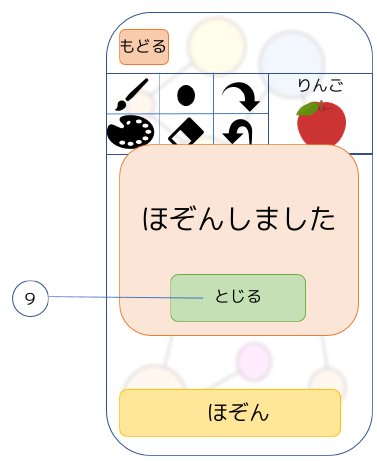
\includegraphics {storage.png}}
    \caption {保存画面のイメージ}
    \label{storage}
    \end{center}
    \end{minipage}
\end{figure}

\begin{enumerate}
  \renewcommand{\labelenumi}{\textcircled{\scriptsize \theenumi}}
\item もどるボタン\\
  もどるボタンをタップすることでおえかきゲーム画面(図\ref{oekaki})に遷移します。
\item ペンのイラストボタン\\
  ペンのイラストボタンをタップすることでペンの種類を変更できます。
\item 黒い丸ボタン\\
  黒い丸ボタンをタップすることでペンの太さを選択できます。
\item 進むボタン\\
  進むボタンをタップすることでイラストが1段階進みます。
\item パレットのイラストボタン\\
  パレットのイラストボタンをタップすることでペンの色を選択できます。
\item 消しゴムのイラストボタン\\
  消しゴムのイラストボタンをタップすることでペンが消しゴムに代わりおえかきを消すことができます。
\item もどるボタン\\
  1段階もどるボタンをタップすることで描いたイラストを1段階もどすことができます。
\item 保存ボタン\\
  保存ボタンをタップすることで図\ref{storage}のように「ほぞんしました」と表示されおえかきが成長記録として保存されます。
\item とじるボタン\\
  図\ref{storage}のとじるボタンをタップすることで図\ref{storage}の表示を閉じます。
\end{enumerate}

\newpage
\subsubsection{おえかき画面}
図\ref{oekaki2}はおえかき画面を示します。\\

\begin{figure}[H]
  \begin{minipage}{0.5\hsize}
    \begin{center}
    \resizebox{8cm}{!}{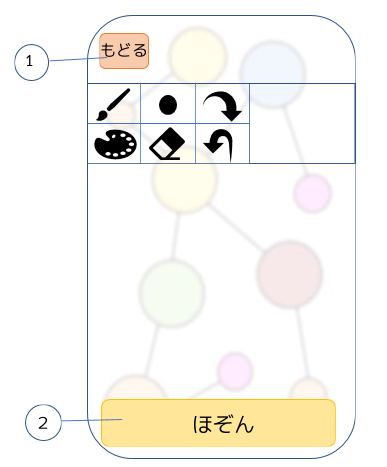
\includegraphics {oekaki2.png}}
    \caption {おえかき画面のイメージ}
    \label{oekaki2}
    \end{center}
  \end{minipage}
  \begin{minipage}{0.5\hsize}
    \begin{center}
    \resizebox{8cm}{!}{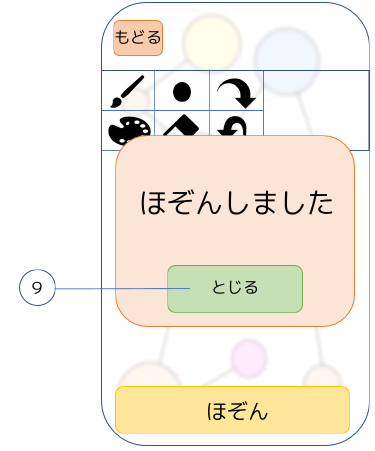
\includegraphics {storage2.png}}
    \caption {保存画面のイメージ}
    \label{storage2}
    \end{center}
    \end{minipage}
\end{figure}

\begin{enumerate}
  \renewcommand{\labelenumi}{\textcircled{\scriptsize \theenumi}}
\item もどるボタン\\
  もどるボタンをタップすることでおえかきゲーム画面(図\ref{oekaki})に遷移します。
\item ペンのイラストボタン\\
  ペンのイラストボタンをタップすることでペンの種類を変更できます。
\item 黒い丸ボタン\\
  黒い丸ボタンをタップすることでペンの太さを選択できます。
\item 進むボタン\\
  進むボタンをタップすることでイラストが1段階進みます。
\item パレットのイラストボタン\\
  パレットのイラストボタンをタップすることでペンの色を選択できます。
\item 消しゴムのイラストボタン\\
  消しゴムのイラストボタンをタップすることでペンが消しゴムに代わりおえかきを消すことができます。
\item 1段階もどるボタン\\
  1段階もどるボタンをタップすることで描いたイラストを1段階もどすことができます。
\item 保存ボタン\\
  保存ボタンをタップすることで図\ref{storage2}のように「ほぞんしました」と表示されおえかきが成長記録として保存されます。
\item とじるボタン\\
  図\ref{storage2}のとじるボタンをタップすることで表示を図\ref{storage2}の表示を閉じます。
\end{enumerate}

\newpage
\subsubsection{おつかいゲーム画面}
図\ref{otukai1}におつかいの詳細画面を示します。\\
おつかいは作りたい料理を選択し、その料理に必要な材料をお店から買ってくるゲームです。\\

\begin{figure}[H]
    \begin{center}
    \resizebox{8cm}{!}{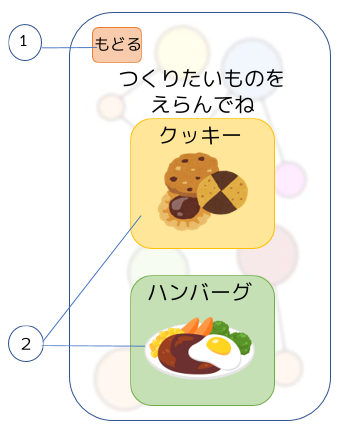
\includegraphics {otukai1.png}}
    \caption {おつかいのイメージ}
    \label{otukai1}
    \end{center}
\end{figure}

\begin{enumerate}
  \renewcommand{\labelenumi}{\textcircled{\scriptsize \theenumi}}
\item もどるボタン\\
  もどるボタンをタップすることでゲーム選択画面(図\ref{game})に遷移します。
\item イラストボタン\\
  図\ref{otukai1}の料理のイラストボタンをタップするとその料理の材料画面(図\ref{material})に遷移します。
\end{enumerate}

\newpage
\subsubsection{材料画面}
図\ref{material}は材料画面を示します。\\

\begin{figure}[H]
    \begin{center}
    \resizebox{8cm}{!}{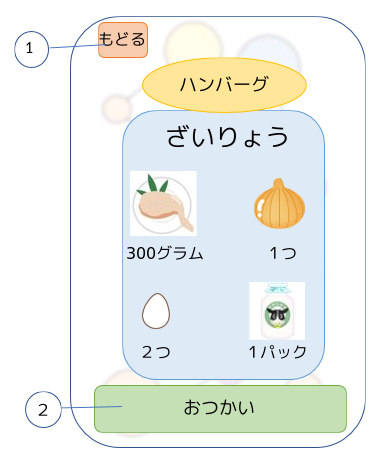
\includegraphics {material.png}}
    \caption {材料画面のイメージ}
    \label{material}
    \end{center}
\end{figure}

\begin{enumerate}
  \renewcommand{\labelenumi}{\textcircled{\scriptsize \theenumi}}
\item もどるボタン\\
  材料画面(図\ref{material})のもどるボタンをタップするとおつかい画面(図\ref{otukai1})へ遷移します。
\item おつかいボタン\\
 おつかいのボタンをタップするとお店の画面(図\ref{shop})へ遷移します。
\end{enumerate}

\newpage
\subsubsection{お店画面}
図\ref{shop}はお店画面を示します。\\

\begin{figure}[H]
    \begin{center}
    \resizebox{8cm}{!}{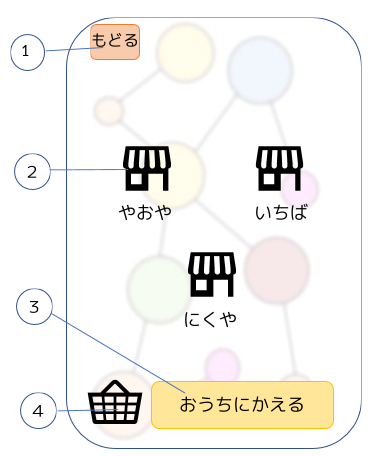
\includegraphics {shop.png}}
    \caption {お店のイメージ}
    \label{shop}
    \end{center}
\end{figure}

\begin{enumerate}
  \renewcommand{\labelenumi}{\textcircled{\scriptsize \theenumi}}
\item もどるボタン\\
  お店画面(図\ref{shop})のもどるボタンをタップすると食材画面(図\ref{material})にもどります。
\item お店のイラストボタン\\
  お店のイラストボタンをタップするとお店に置いている食材画面(図\ref{shop_material})へ遷移します。
\item おうちにかえるボタン\\
  おうちにかえるをタップするとおうち画面(図\ref{myhome})へ遷移します。
\item かごのイラストボタン\\
  かごのイラストをタップすると図\ref{have}の材料確認画面に遷移し、持っている材料を確認することができます。
\end{enumerate}

\newpage
\subsubsection{材料確認画面}
図\ref{have}は材料確認画面を示します。\\

\begin{figure}[H]
    \begin{center}
    \resizebox{8cm}{!}{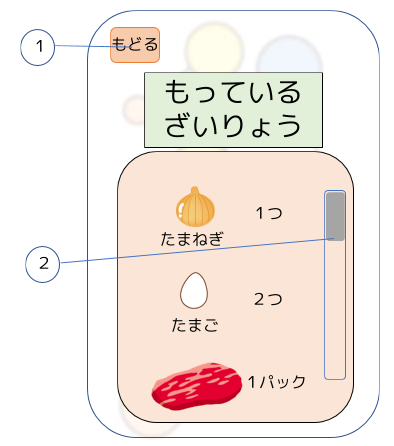
\includegraphics {have.png}}
    \caption {材料確認画面のイメージ}
    \label{have}
    \end{center}
\end{figure}

\begin{enumerate}
  \renewcommand{\labelenumi}{\textcircled{\scriptsize \theenumi}}
\item もどるボタン\\
  材料確認画面(図\ref{have})のもどるボタンをタップするとお店画面(図\ref{shop})にもどります。
\item スクロールバー\\
  スクロールバーをスクロールすることで持っている材料を閲覧できます。
\end{enumerate}

\newpage
\subsubsection{食材画面}
図\ref{shop_material}は食材画面を示します。\\

\begin{figure}[H]
    \begin{center}
    \resizebox{8cm}{!}{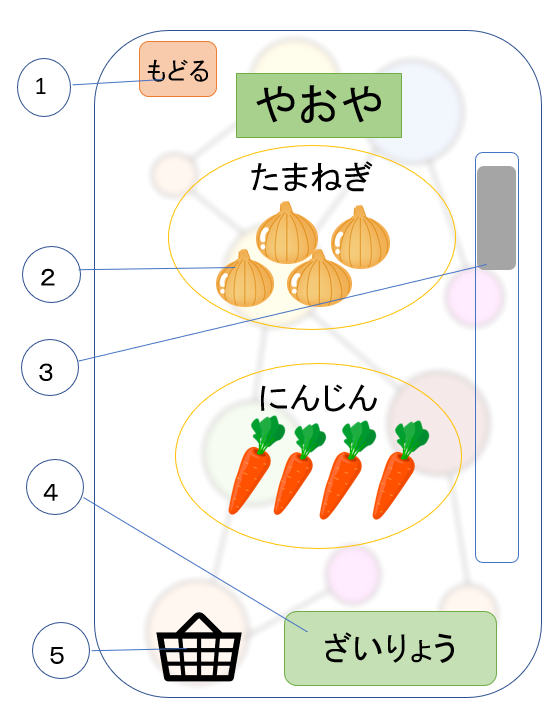
\includegraphics {shop_material.png}}
    \caption {食材画面のイメージ}
    \label{shop_material}
    \end{center}
\end{figure}

\begin{enumerate}
  \renewcommand{\labelenumi}{\textcircled{\scriptsize \theenumi}}
\item もどるボタン\\
  食材画面(図\ref{shop_material})のもどるボタンをタップするとお店画面(図\ref{shop})にもどります。
\item 食材のイラストボタン\\
  食材のイラストボタンをタップすることで材料の中にタップした食材が1つずつ格納されます。
\item スクロールバー\\
  スクロールバーをスクロールすることでその他の食材を閲覧できます。
\item ざいりょうボタン\\
  ざいりょうをタップすると作りたい料理の材料を確認できます。
\item かごのイラストボタン\\
  かごのイラストをタップすると図\ref{have}の材料確認画面に遷移し、持っている材料を確認することができます。
\end{enumerate}

\newpage
\subsubsection{おうち画面}
図\ref{myhome}はおうち画面を示します。\\


\begin{figure}[H]
 \begin{minipage}{0.5\hsize}
   \begin{center}
   \resizebox{8cm}{!}{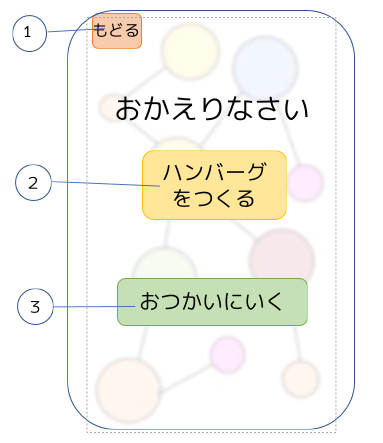
\includegraphics {go_home.png}}
   \caption{おうち画面のイメージ}
   \label{myhome}
  \end{center}
 \end{minipage}
 \begin{minipage}{0.5\hsize}
  \begin{center}
   \resizebox{8cm}{!}{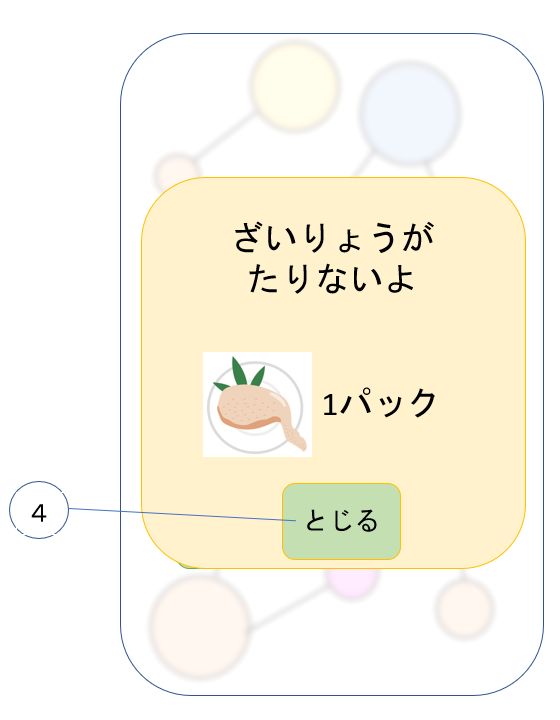
\includegraphics {lack.png}}
   \caption{材料が足りない場合のイメージ}
   \label{otukai6}
  \end{center}
 \end{minipage}
\end{figure}

\begin{enumerate}
  \renewcommand{\labelenumi}{\textcircled{\scriptsize \theenumi}}
\item もどるボタン\\
  おうち画面(図\ref{myhome})のもどるボタンをタップするとお店画面(図\ref{shop})にもどります。
\item つくるボタン\\
  材料が揃っている場合、おうち画面(図\ref{myhome})のつくるボタンをタップするとできあがり画面(図\ref{completion})へ遷移します。材料が揃っていない場合、図\ref{otukai6}のように「ざいりょうがたりないよ」と表示されます。
\item おつかいボタン\\
  おうち画面(図\ref{myhome})のおつかいにいくをタップするとお店の画面(図\ref{shop})へ遷移します。
\item とじるボタン\\
  図\ref{otukai6}の閉じるボタンをタップするとおうち画面(図\ref{myhome})へ遷移します。
\end{enumerate}

\newpage
\subsubsection{できあがり画面}
図\ref{completion}はできあがり画面を示します。\\

\begin{figure}[H]
    \begin{center}
    \resizebox{8cm}{!}{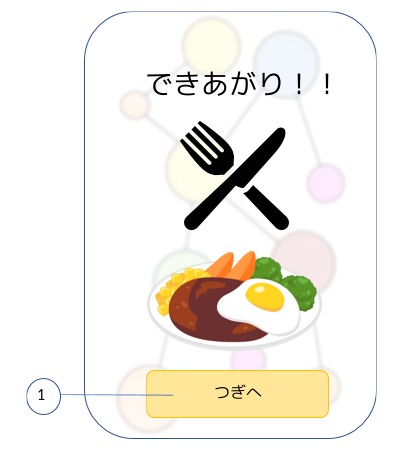
\includegraphics {completion.png}}
    \caption {できあがり画面のイメージ}
    \label{completion}
    \end{center}
\end{figure}

\begin{enumerate}
  \renewcommand{\labelenumi}{\textcircled{\scriptsize \theenumi}}
\item つぎへ\\
  つぎへをタップすることでおつかいのゲーム画面(図\ref{otukai1})に遷移します。
\end{enumerate}


% 成長記録%
\newpage
\subsection{成長記録}\label{grow}
図\ref{Grow}に、成長記録起動時の画面を示します。
成長記録は、自分の撮影した子どもの写真やゲームの記録を保存し、閲覧及び共有することができます。

\begin{figure}[H]
    \begin{center}
    \resizebox{8cm}{!}{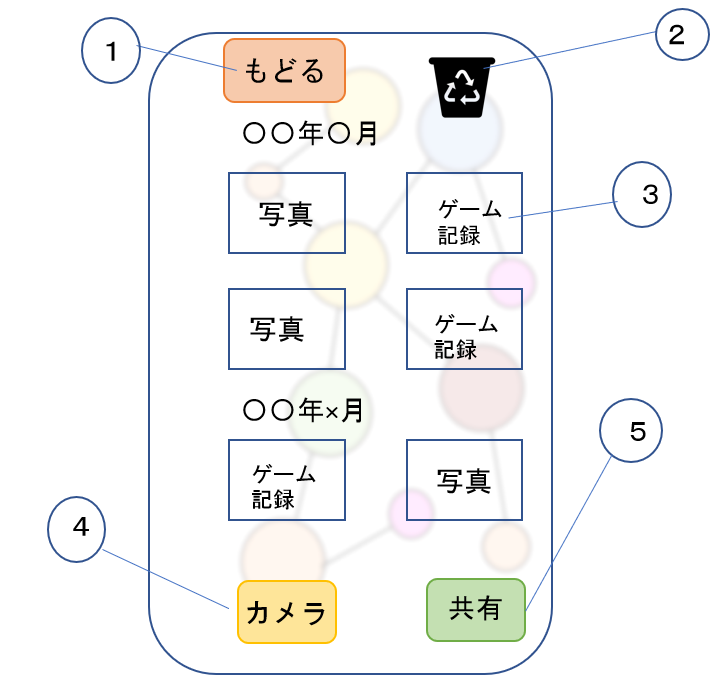
\includegraphics {Albam1.png}}
    \caption {成長記録の画面のイメージ}
    \label{Grow}
    \end{center}
\end{figure}

\begin{enumerate}
  \renewcommand{\labelenumi}{\textcircled{\scriptsize \theenumi}}
  \item もどるボタン\\
       タップすると、メインメニュー画面(図\ref{honjo_main})に戻ります。
  \item ゴミ箱ボタン\\
      タップすると、選択画面(図\ref{deleter})に遷移し、不要になった写真やゲーム記録を選択する事で削除できます。選択した写真などには左上にチェックマークが表示されます。選択後は一度、確認画面(図\ref{checker})が表示されます。「はい」をタップすると消去され、「いいえ」をタップするとキャンセルされます。
  \item 写真及びゲーム記録\\
       撮影した写真やゲームの記録を閲覧することができます。各写真や記録をタップするとアルバム画面(図\ref{Albam})に遷移します。
  \item カメラボタン\\
        撮影したいときに使用するボタンです。ボタンをタップするとシステム内からカメラを起動し写真を撮影することができます。
  \item 共有ボタン \label{enum:share}\\
        写真やゲームの記録を共有したい時に使用するボタンです。ボタンをタップすると外部アプリ(Twitter)を起動し共有することができます。
\end{enumerate}
\begin{figure}[H]
 \begin{minipage}{0.5\hsize}
   \begin{center}
   \resizebox{8cm}{!}{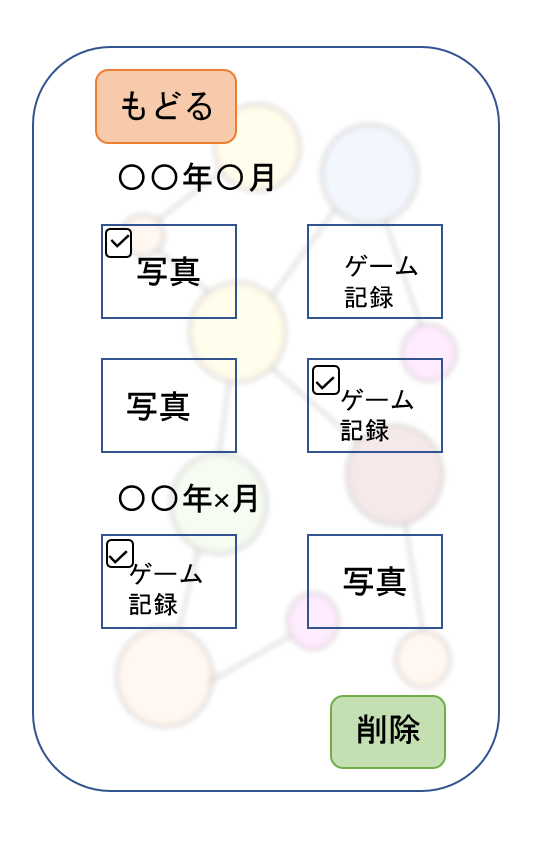
\includegraphics {deleter.png}}
   \caption{選択画面のイメージ}
   \label{deleter}
  \end{center}
 \end{minipage}
 \begin{minipage}{0.5\hsize}
  \begin{center}
   \resizebox{8cm}{!}{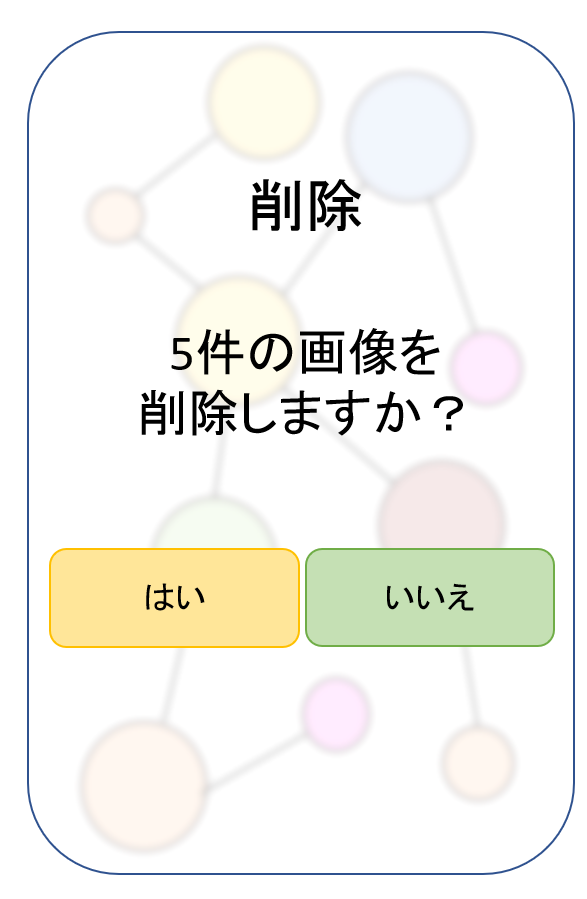
\includegraphics {checker.png}}
   \caption{確認画面のイメージ}
   \label{checker}
  \end{center}
 \end{minipage}
\end{figure}

\newpage
\subsubsection{アルバム画面}
写真をタップしたときに拡大表示される画面(図\ref{Albam})に遷移します。
写真や記録は拡大して表示されます。また、共有ボタンもありここから外部アプリ(Twitter)を起動し共有することができます。

\begin{figure}[H]
    \begin{center}
    \resizebox{8cm}{!}{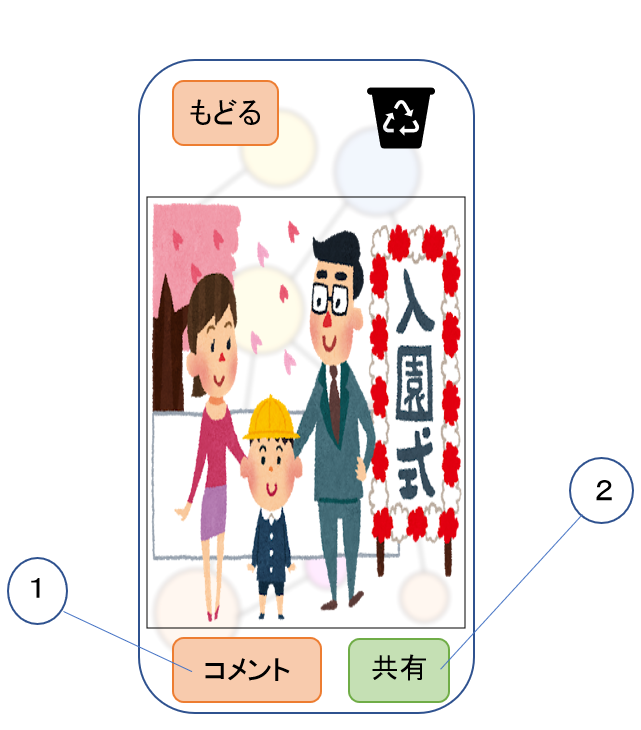
\includegraphics {Albam2.png}}
    \caption {アルバム画面のイメージ}
    \label{Albam}
    \end{center}
\end{figure}

\begin{enumerate}
  \renewcommand{\labelenumi}{\textcircled{\scriptsize \theenumi}}
  \item コメントボタン\\
    アルバムに保存された写真や記録にはコメントボタンを押すことによりコメント入力画面(図\ref{Comment})に遷移し、コメントを残すことができます。
  \item 共有ボタン\\
    写真やゲームの記録を共有したい時に使用するボタンです。ボタンをタップすると外部アプリ(Twitter)を起動し共有することができます。
\end{enumerate}

\begin{figure}[H]
    \begin{center}
    \resizebox{8cm}{!}{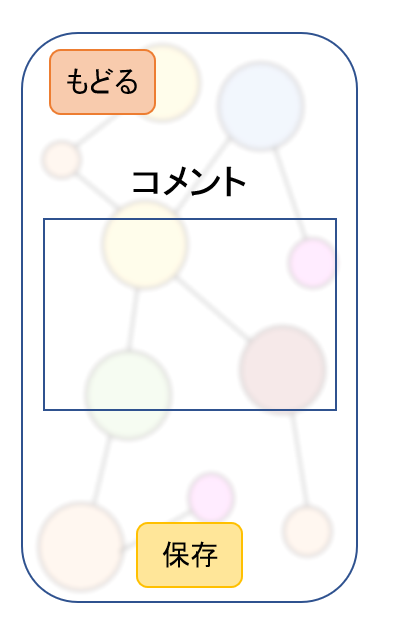
\includegraphics {comment.png}}
    \caption {コメント入力画面のイメージ}
    \label{Comment}
    \end{center}
\end{figure}

\begin{enumerate}
  \renewcommand{\labelenumi}{\textcircled{\scriptsize \theenumi}}
  \item もどるボタン\\
     もどるボタンをタップすると、アルバム画面(図\ref{Albam})に戻ります。
  \item コメント入力欄\\
     この枠内に残したいコメントを書き記すことができます。
  \item 保存ボタン\\
     保存ボタンをタップすると、編集した写真を保存することができます。
\end{enumerate}

\subsubsection{カメラ}
カメラボタンを押すことによりカメラ(図\ref{Camera})を起動します。
カメラを使用して撮影するときに使用されます。ここで撮影された写真はアルバムとして保存され図\ref{Albam}のように閲覧、共有することができます。


\begin{figure}[H]
    \begin{center}
    \resizebox{12cm}{!}{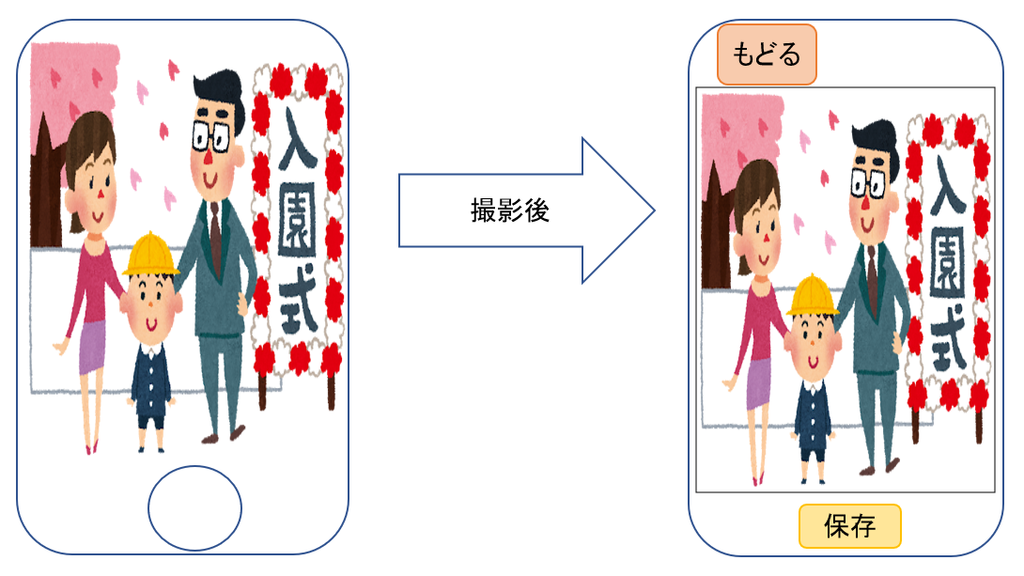
\includegraphics {Camera.png}}
    \caption {カメラ画面のイメージ}
    \label{Camera}
    \end{center}
\end{figure}


\subsubsection{共有}
写真や記録を共有したいときに使用されます。共有は外部アプリであるTwitterで行われます。共有するためには成長記録画面(図\ref{Grow})とアルバム画面(図\ref{Albam})についている共有ボタンをタップすることで起動することができます。

%質問箱%
\subsection{子育て窓口}
図\ref{honjo_CR_Window}に、子育て窓口の画面を示します。
子育てにおける不安・疑問を、検索や投稿を行うことによって解決するために使用されます。

図\ref{honjo_CR_Window}に示す番号と対応させる形式で、以下にその役割を示します。

\begin{figure}[H]
    \begin{center}
    \resizebox{8cm}{!}{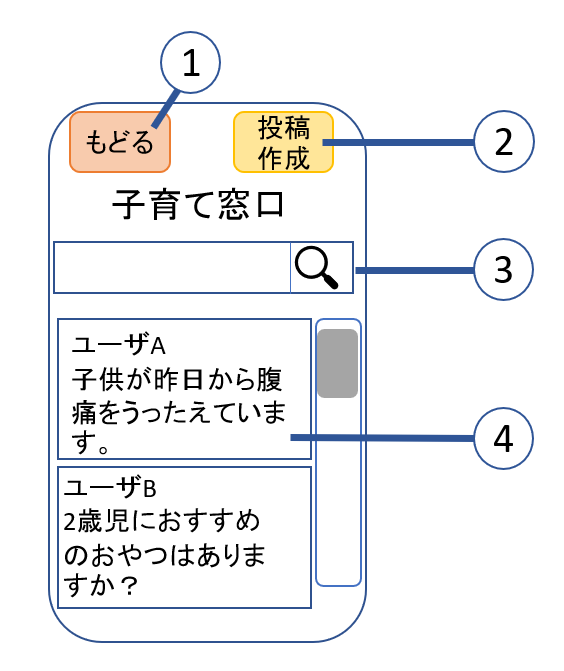
\includegraphics {honjo_CR_Window.png}}
    \caption {子育て窓口の画面のイメージ}
    \label{honjo_CR_Window}
    \end{center}
\end{figure}

\begin{enumerate}
  \renewcommand{\labelenumi}{\textcircled{\scriptsize \theenumi}}
  \item もどるボタン\\
        もどるボタンをタップすると、メインメニュー画面(図\ref{honjo_main})へ遷移します。
  \item 質問投稿作成ボタン\\
        質問投稿をしたい時に押すボタンです。ペンのボタンをタップすると、質問を行うための投稿画面(図\ref{honjo_CR_Contribution})へ遷移します。
  \item 質問の検索欄\\
        ユーザが子育て窓口内に投稿されたものを検索するために使用します。矩形領域をタップするとキーボードが開き、入力することが可能になります。
  \item 質問の一覧表示\\
        子育て窓口に投稿された質問が一覧表示されます。質問が書かれている矩形領域をタップすると質問の詳細画面(図\ref{honjo_CR_Answer})へ遷移します。
\end{enumerate}


\subsubsection{質問投稿画面}
図\ref{honjo_CR_Contribution}に、質問の投稿画面を示します。
質問の投稿を行うために使用されます。

図\ref{honjo_CR_Contribution}に示す番号と対応させる形式で、以下にその役割を示します。

\begin{figure}[H]
    \begin{center}
    \resizebox{8cm}{!}{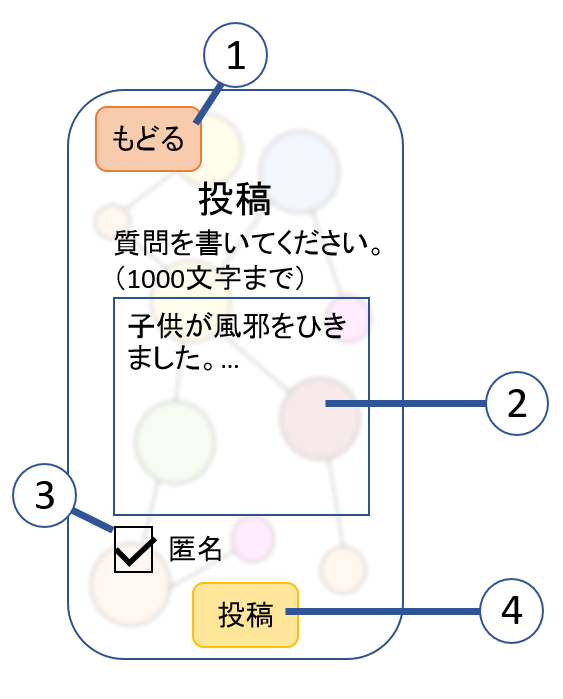
\includegraphics {honjo_CR_Contribution.png}}
    \caption {質問投稿画面のイメージ}
    \label{honjo_CR_Contribution}
    \end{center}
\end{figure}

\begin{enumerate}
  \renewcommand{\labelenumi}{\textcircled{\scriptsize \theenumi}}
  \item もどるボタン\\
        もどるボタンをタップすると、子育て窓口の画面(図\ref{honjo_CR_Window})へ遷移します。
  \item 質問内容の入力欄\\
        ユーザが質問の内容を書き込むための欄です。矩形領域をタップするとキーボードが開き、入力することが可能になります。
  \item 匿名チェックボックス\\
        チェックボックスをタップして、チェックが入ると、匿名で回答を投稿することが出来ます。
  \item 投稿ボタン\\
        質問を入力欄に書き終えて投稿をしたい時に押すボタンです。質問投稿完了画面(図\ref{honjo_CR_CompleteContribution})へ遷移します。
\end{enumerate}


\newpage
\subsubsection{質問投稿完了画面}
図\ref{honjo_CR_CompleteContribution}に、質問の投稿完了画面を示します。
質問の投稿が正常に完了したことを通知するために使用されます。

図\ref{honjo_CR_CompleteContribution}に示す番号と対応させる形式で、以下にその役割を示します。

\begin{figure}[H]
    \begin{center}
    \resizebox{12cm}{!}{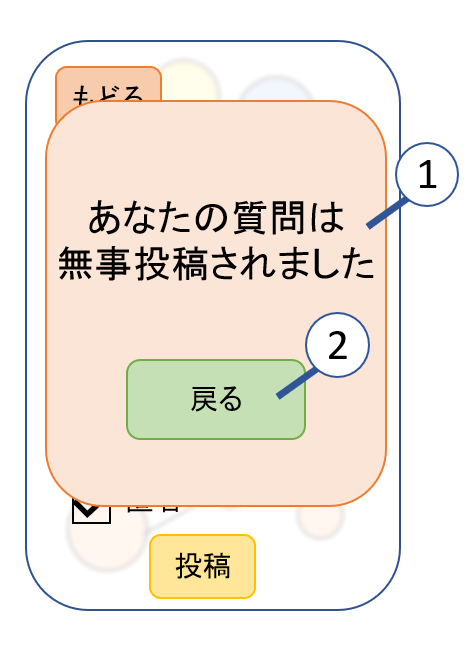
\includegraphics{honjo_CR_CompleteContribution.png}}
    \caption {質問投稿完了画面のイメージ}
    \label{honjo_CR_CompleteContribution}
    \end{center}
\end{figure}

\begin{enumerate}
  \renewcommand{\labelenumi}{\textcircled{\scriptsize \theenumi}}
  \item ステータス\\
        ユーザの質問投稿が正常に完了したかを通知します。何らかのエラーが発生し投稿できなかった場合は、右図のようになります。
  \item もどるボタン\\
        もどるボタンをタップすると、子育て窓口の画面(図\ref{honjo_CR_Window})へ遷移します。
\end{enumerate}


\newpage
\subsubsection{質問の詳細画面}
図\ref{honjo_CR_Answer}に、質問の詳細画面を示します。
質問の詳細を閲覧、またその質問に対して回答を行うために使用されます。

図\ref{honjo_CR_Answer}に示す番号と対応させる形式で、以下にその役割を示します。

\begin{figure}[H]
    \begin{center}
    \resizebox{8cm}{!}{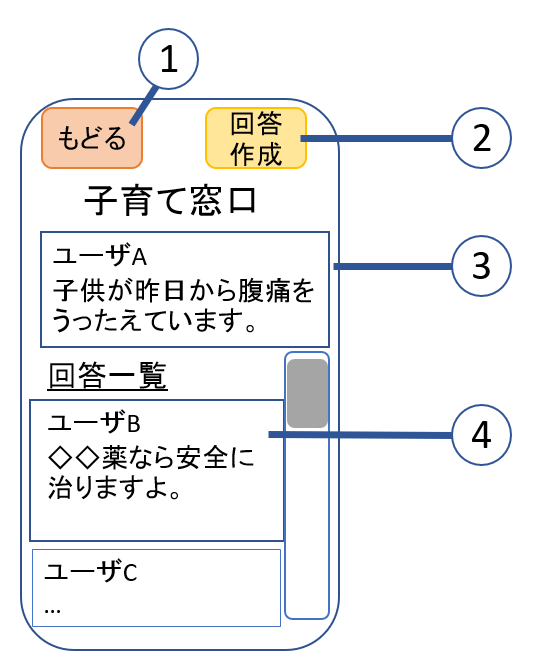
\includegraphics {honjo_CR_Answer.png}}
    \caption {質問の詳細画面のイメージ}
    \label{honjo_CR_Answer}
    \end{center}
\end{figure}

\begin{enumerate}
  \renewcommand{\labelenumi}{\textcircled{\scriptsize \theenumi}}
  \item もどるボタン\\
        もどるボタンをタップすると、子育て窓口の画面(図\ref{honjo_CR_Window})へ遷移します。
  \item 回答作成ボタン\\
        この質問に対する回答を作成するためのボタンです。タップすると回答作成画面(図\ref{honjo_CR_CreateAnswer})へ遷移します。
  \item 質問内容\\
        質問内容の全文を表示します。
  \item 回答内容\\
        回答内容の全文を表示します。複数回答がある場合は下にスクロールすることで閲覧が可能になります。
\end{enumerate}

\newpage
\subsubsection{回答作成画面}
図\ref{honjo_CR_CreateAnswer}に、回答の作成画面を示します。
ある質問に対する回答を行うために使用されます。

図\ref{honjo_CR_CreateAnswer}に示す番号と対応させる形式で、以下にその役割を示します。

\begin{figure}[H]
    \begin{center}
    \resizebox{10cm}{!}{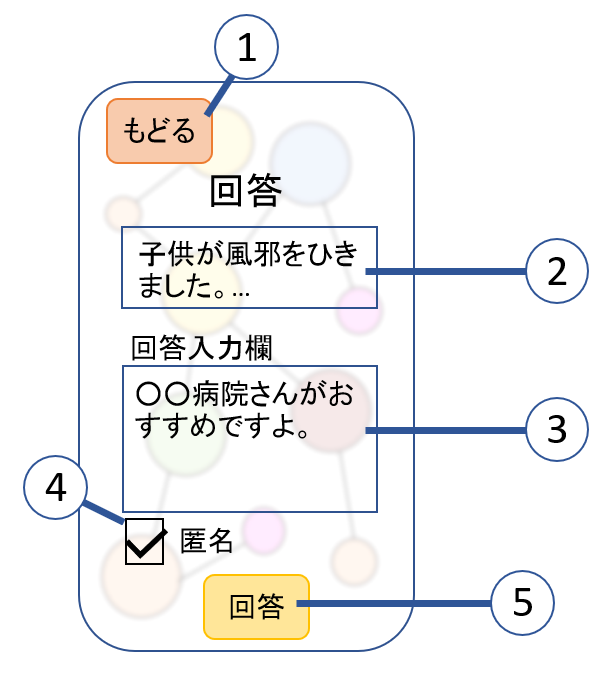
\includegraphics {honjo_CR_CreateAnswer.png}}
    \caption {回答作成画面のイメージ}
    \label{honjo_CR_CreateAnswer}
    \end{center}
\end{figure}

\begin{enumerate}
  \renewcommand{\labelenumi}{\textcircled{\scriptsize \theenumi}}
  \item もどるボタン\\
        もどるボタンをタップすると、質問の詳細画面(図\ref{honjo_CR_Answer})へ遷移します。
  \item 質問内容\\
        質問内容の全文を表示します。
  \item 回答内容の入力欄\\
        ユーザが回答内容を入力するための欄です。矩形領域をタップするとキーボードが開き、入力することが可能になります。
  \item 匿名チェックボックス\\
        チェックボックスをタップして、チェックが入ると、匿名で回答を投稿することが出来ます。
  \item 回答投稿ボタン\\
        回答を入力欄に書き終えて投稿をしたい時に押すボタンです。回答投稿完了画面(図\ref{honjo_CR_CompleteAnswer})へ遷移します。
\end{enumerate}

\newpage
\subsubsection{回答投稿完了画面}
図\ref{honjo_CR_CompleteAnswer}に、質問の投稿完了画面を示します。
質問の投稿が正常に完了したことを通知するために使用されます。

図\ref{honjo_CR_CompleteAnswer}に示す番号と対応させる形式で、以下にその役割を示します。

\begin{figure}[H]
    \begin{center}
    \resizebox{12cm}{!}{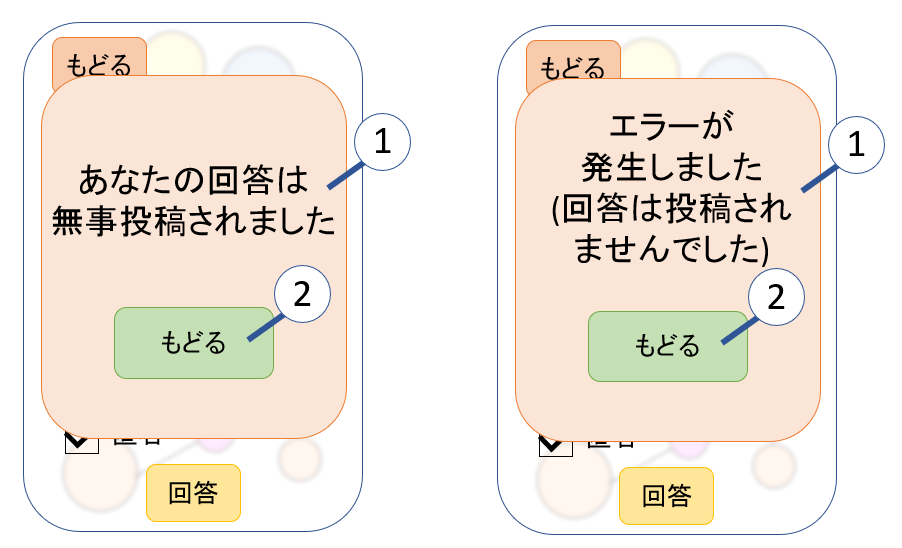
\includegraphics {honjo_CR_CompleteAnswer.png}}
    \caption {回答投稿完了画面のイメージ}
    \label{honjo_CR_CompleteAnswer}
    \end{center}
\end{figure}

\begin{enumerate}
  \renewcommand{\labelenumi}{\textcircled{\scriptsize \theenumi}}
  \item ステータス\\
        ユーザの回答投稿が正常に完了したかを通知します。何らかのエラーが発生し投稿できなかった場合は、右図のようになります。
  \item もどるボタン\\
        もどるボタンをタップすると、子育て窓口の画面(図\ref{honjo_CR_Window})へ遷移します。
\end{enumerate}

%変更・問い合わせ%
\newpage
\subsection{設定}
図\ref{configuration}は設定画面を示します。\\
設定では、管理者への問い合わせやアカウントの設定、ゲームのパスワード設定をすることができます。

\begin{figure}[H]
    \begin{center}
    \resizebox{8cm}{!}{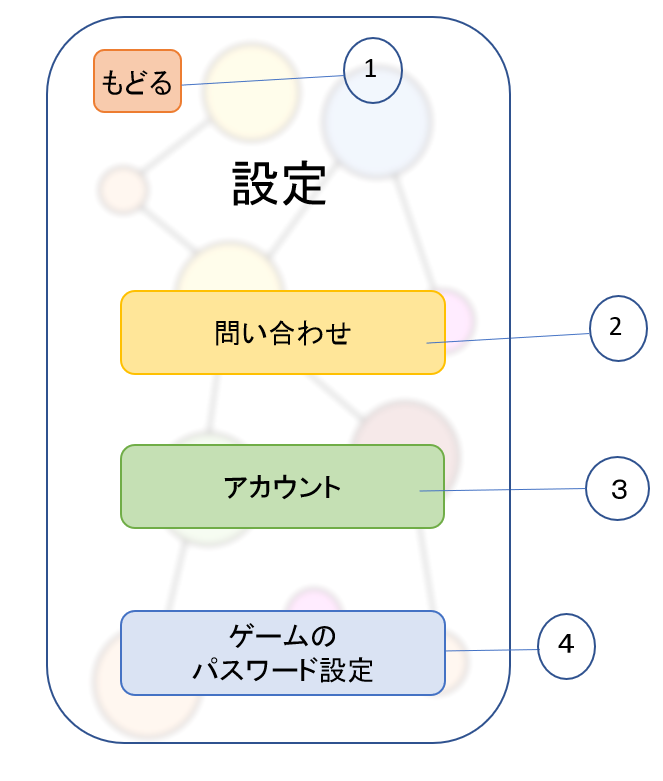
\includegraphics {configuration.png}}
    \caption {設定画面のイメージ}
    \label{configuration}
    \end{center}
\end{figure}

\begin{enumerate}
  \renewcommand{\labelenumi}{\textcircled{\scriptsize \theenumi}}
\item もどるボタン\\
  タップすると、メインメニュー画面(図\ref{honjo_main})へ遷移します。
\item 問い合わせボタン\\
  タップすることで問い合わせのメールアドレスと問い合わせに必要な情報を記載したページ(図\ref{inquiry})に遷移します。
\item アカウントボタン\\
  タップすると変更と削除の画面(図\ref{account})に遷移します。
\item ゲームのパスワード設定ボタン\\
 タップするとゲーム画面からメニュー画面に遷移するためのパスワード設定画面(図\ref{passwordchange})に遷移します。
\end{enumerate}

\begin{figure}[H]
    \begin{center}
    \resizebox{8cm}{!}{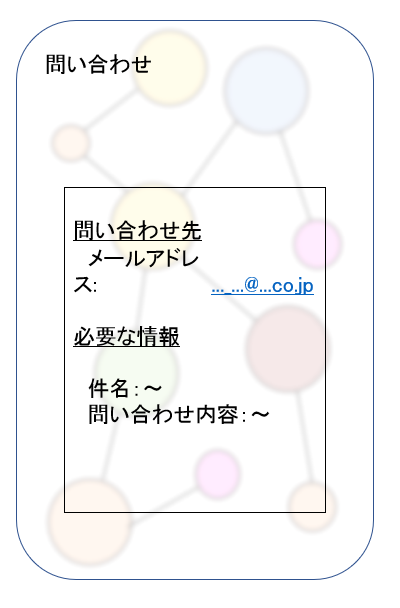
\includegraphics {inquiry.png}}
    \caption {問い合わせ画面のイメージ}
    \label{inquiry}
    \end{center}
\end{figure}

\begin{enumerate}
  \renewcommand{\labelenumi}{\textcircled{\scriptsize \theenumi}}
\item もどるボタン\\
  タップすると、設定画面(図\ref{configuration})へ遷移します。
\end{enumerate}

\newpage
\subsubsection{アカウント}
図\ref{account}はアカウントの設定画面を示します。\\
アカウントの設定ではアカウントの変更と削除ができます。

\begin{figure}[H]
    \begin{center}
    \resizebox{8cm}{!}{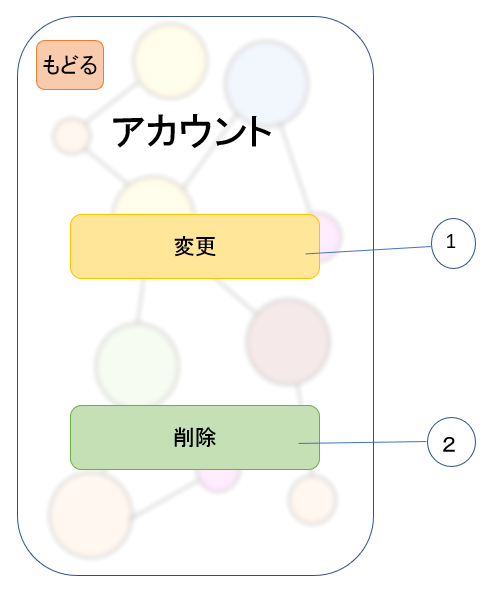
\includegraphics {account.png}}
    \caption {アカウント画面のイメージ}
    \label{account}
    \end{center}
\end{figure}

\begin{enumerate}
  \renewcommand{\labelenumi}{\textcircled{\scriptsize \theenumi}}
\item もどるボタン\\
  タップすると、設定画面(図\ref{configuration})へ遷移します。
\item 変更\\
  タップするとニックネームと地域の設定画面(図\ref{change})に遷移します。
\item 削除\\
  タップすると削除をするか確認する画面(図\ref{delete})に遷移します。
\end{enumerate}

\newpage
\subsubsection{変更}
図\ref{change}はアカウントの変更画面を示します。\\
変更画面では、ニックネームと地域の変更ができます。

\begin{figure}[H]
  \begin{center}
    \resizebox{8cm}{!}{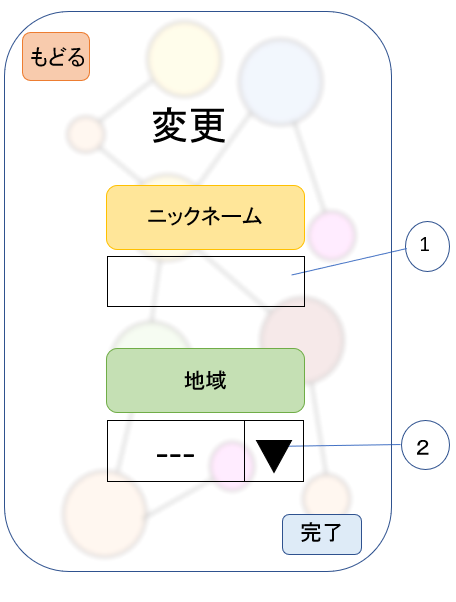
\includegraphics {change.png}}
    \caption {変更画面のイメージ}
    \label{change}
  \end{center}
\end{figure}

\begin{enumerate}
  \renewcommand{\labelenumi}{\textcircled{\scriptsize \theenumi}}
\item もどるボタン\\
  タップすると、アカウント画面(図\ref{account})へ遷移します。
\item ニックネーム入力欄\\
  タップするとキーボードが開き、入力することが可能になります。
\item 居住地域の選択欄\\
  タップすると都道府県の一覧が表示され、選択することができます。
\item 完了ボタン\\
  タップすると、変更内容を保存してアカウント画面(図\ref{account})へ遷移します。
\end{enumerate}


\newpage
\subsubsection{削除}
図\ref{delete}はアカウントの削除画面を示します。\\

\begin{figure}[H]
    \begin{center}
    \resizebox{8cm}{!}{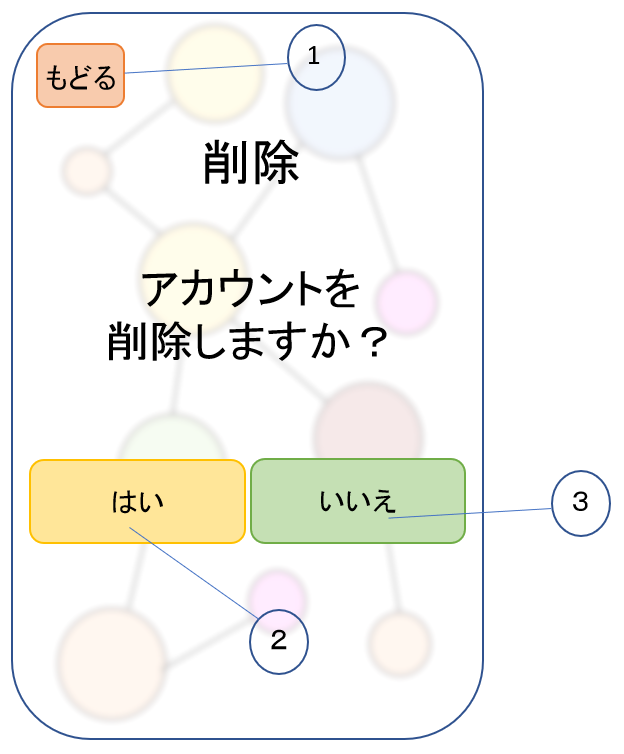
\includegraphics {delete.png}}
    \caption {削除画面のイメージ}
    \label{delete}
    \end{center}
\end{figure}

\begin{enumerate}
  \renewcommand{\labelenumi}{\textcircled{\scriptsize \theenumi}}
\item もどるボタン\\
  タップすると、アカウント画面(図\ref{account})へ遷移します。
\item はい\\
  タップすると削除が完了し、アカウント削除完了画面(図\ref{check})へ遷移します。
\item いいえ\\
  タップするとアカウントの設定画面(図\ref{account})に遷移します。
\end{enumerate}

\begin{figure}[H]
    \begin{center}
    \resizebox{8cm}{!}{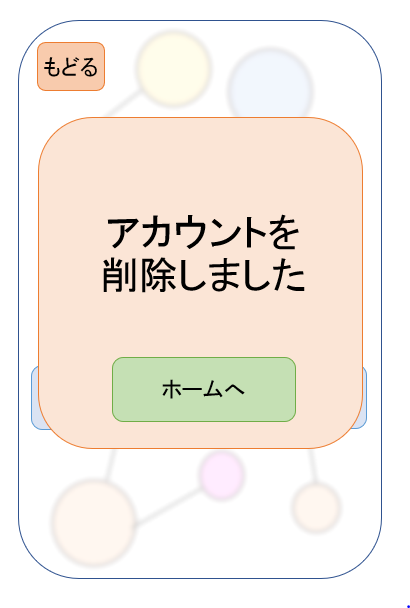
\includegraphics {check.png}}
    \caption {アカウント削除完了画面のイメージ}
    \label{check}
    \end{center}
\end{figure}

\begin{enumerate}
  \renewcommand{\labelenumi}{\textcircled{\scriptsize \theenumi}}
\item ホームへボタン\\
  タップすると、初期設定画面(図\ref{honjo_setup})へ遷移します。
\end{enumerate}

\newpage
\subsubsection{ゲームのパスワード設定}
図\ref{passwordchange}はゲーム画面からメニュー画面へ遷移するためのパスワードの設定画面を示します。\\

\begin{figure}[H]
    \begin{center}
    \resizebox{8cm}{!}{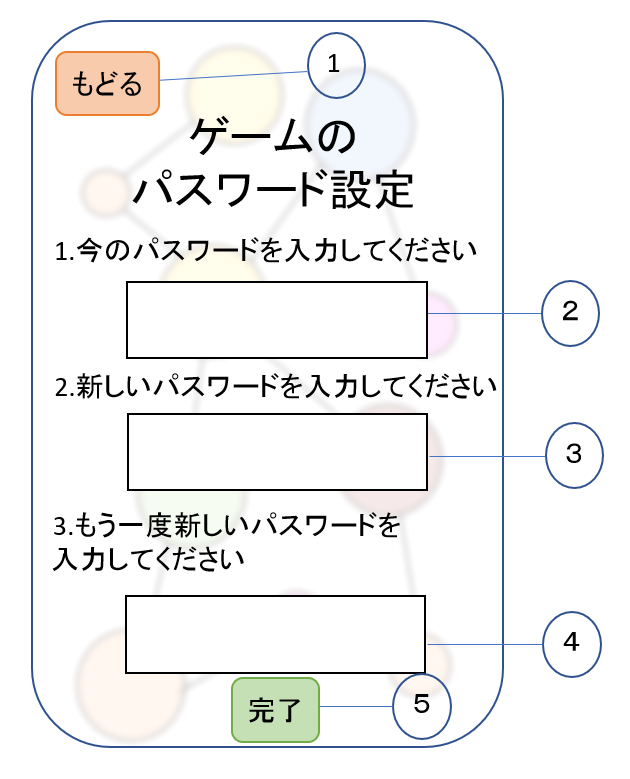
\includegraphics {passwordchange.png}}
    \caption {ゲームのパスワード設定画面のイメージ}
    \label{passwordchange}
    \end{center}
\end{figure}

\begin{enumerate}
  \renewcommand{\labelenumi}{\textcircled{\scriptsize \theenumi}}
\item もどるボタン\\
  タップすると、設定画面(図\ref{configuration})へ遷移します。
\item パスワード入力1\\
  タップするとキーボードが開くので、設定したいパスワードを入力します。
\item パスワード入力2\\
  タップするとキーボードが開くので、パスワードの入力間違いがないようもう一度パスワードを入力します。
\item 完了ボタン\\
  タップするとパスワード設定が完了し、パスワード設定完了画面(図\ref{passwordchange_check})へ遷移します。ただし、パスワード入力1及びパスワード入力2の入力が済まない限り、タップすることができません。
\end{enumerate}

\begin{figure}[H]
    \begin{center}
    \resizebox{8cm}{!}{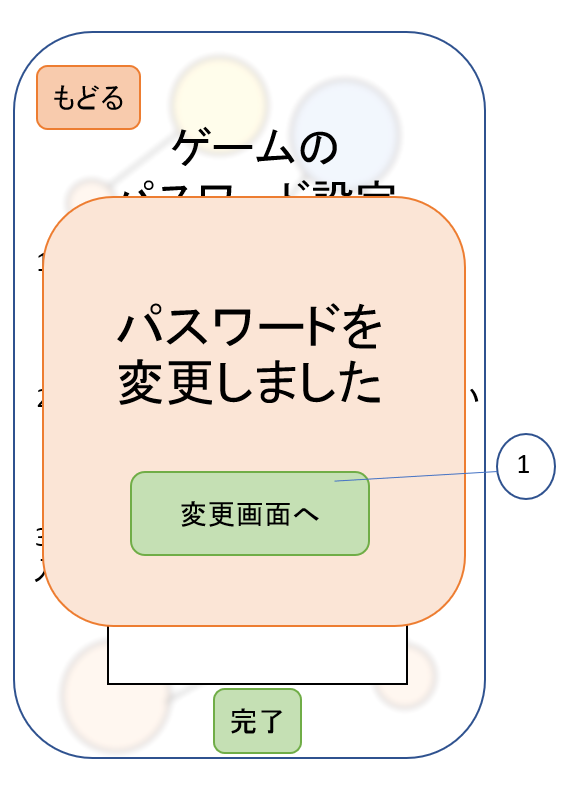
\includegraphics {passwordchange_check.png}}
    \caption {パスワード設定完了画面のイメージ}
    \label{passwordchange_check}
    \end{center}
\end{figure}

\begin{enumerate}
  \renewcommand{\labelenumi}{\textcircled{\scriptsize \theenumi}}
\item 設定画面へボタン\\
  タップすると、設定画面(図\ref{configuration})へ遷移します。
\end{enumerate}

\newpage
\section{データテーブル設計}

以下に本システムで用いるデータテーブルを示します。\\
表\ref{tbl: user}はユーザ情報を示しており、親の情報を格納しています。\\

\begin{table}[H]
    \caption{ユーザ情報}
    \label{tbl: user}
    \begin{center}
        \begin{tabular}{|c|c|c|c|c|} \hline
            属性 & データ型 & データ長 & SQLite & key:Table名\\ \hline \hline
            UserID & 半角英数字型 & 6文字固定長 & TEXT & PK\\ \hline
            Name & 全角文字型 & 10文字可変長 & TEXT & \\ \hline
            Area & 全角文字型 & 5文字可変長 & TEXT & \\ \hline
        \end{tabular}
    \end{center}
\end{table}


表\ref{tbl: question}~表\ref{tbl: date}では、質問箱に関するデータを示しています。表\ref{tbl: question}では質問と質問者の関連付けを、表\ref{tbl: answer}では回答と回答者の関連付けを行い、質問と回答の管理を行っています。\\
また、表\ref{tbl: qcontents}では質問内容を、表\ref{tbl: acontents}では回答内容を、表\ref{tbl: date}では日付の管理を行っています。\\
\begin{table}[H]
    \caption{質問}
    \label{tbl: question}
    \begin{center}
        \begin{tabular}{|c|c|c|c|c|} \hline
            属性 & データ型 & データ長 & SQLite & key:Table名\\ \hline \hline
            QID & 半角英数字型 & 8文字固定長 & TEXT & PK\\ \hline
            UserID & 半角英数字型 & 6文字固定長 & TEXT & FK:親ユーザ情報\\ \hline
            QcontentsID & 半角英数字型 & 10文字固定長 & TEXT & FK:質問内容\\ \hline
            DateID & 半角英数字型 & 8文字固定長 & TEXT & FK:日付\\ \hline
        \end{tabular}
    \end{center}
\end{table}

\begin{table}[H]
    \caption{回答}
    \label{tbl: answer}
    \begin{center}
        \begin{tabular}{|c|c|c|c|c|} \hline
            属性 & データ型 & データ長 & SQLite & key:Table名\\ \hline \hline
            AID & 半角英数字型 & 8文字固定長 & TEXT & PK\\ \hline
            QID & 半角英数字型 & 8文字固定長 & TEXT & FK:質問\\ \hline
            UserID & 半角英数字型 & 6文字固定長 & TEXT & FK:親ユーザ情報\\ \hline
            AcontentsID & 半角英数字型 & 10文字固定長 & TEXT & FK:回答内容\\ \hline
            DateID & 半角英数字型 & 8文字固定長 & TEXT & FK:日付\\ \hline
        \end{tabular}
    \end{center}
\end{table}

\begin{table}[H]
    \caption{質問内容}
    \label{tbl: qcontents}
    \begin{center}
        \begin{tabular}{|c|c|c|c|c|} \hline
           属性 & データ型 & データ長 & SQLite & key:Table名\\ \hline \hline
            QcontentsID & 半角英数字型 & 10文字固定長 & TEXT & PK\\ \hline
            Qcontents & 全角文字型 & 1000文字可変長 & TEXT & \\ \hline
        \end{tabular}
    \end{center}
\end{table}


\begin{table}[H]
    \caption{回答内容}
    \label{tbl: acontents}
    \begin{center}
        \begin{tabular}{|c|c|c|c|c|} \hline
            属性 & データ型 & データ長 & SQLite & key:Table名\\ \hline \hline
            AcontentsID & 半角英数字型 & 10文字固定長 & TEXT & PK\\ \hline
            Acontents & 全角文字型 & 1000文字可変長 & TEXT & \\ \hline
        \end{tabular}
    \end{center}
\end{table}

\begin{table}[H]
    \caption{日付}
    \label{tbl: date}
    \begin{center}
        \begin{tabular}{|c|c|c|c|c|} \hline
            属性 & データ型 & データ長 & SQLite & key:Table名\\ \hline \hline
            DateID & 半角英数字型 & 8文字固定長 & TEXT & PK\\ \hline
            Date & 日付型 & 20文字固定長 & NUMERIC & \\ \hline
        \end{tabular}
    \end{center}
\end{table}


また、表\ref{tbl: datatable}に上記のデータテーブルに対する操作を示します。ユーザ情報はユーザ側と管理者側の両方で編集できるようにします。質問と回答のテーブルはユーザが作成を行い、削除は管理者側が行えるようにします。質問内容と回答内容は内容を修正できるようにユーザが更新できるようにしておきます。日付は自動で保存されるので参照のみできるようにします。

\begin{table}[H]
    \caption{各種データテーブルに対する操作}
    \label{tbl: datatable}
    \begin{center}
        \begin{tabular}{|l||c|c|c|c||c|c|c|c|} \hline
             & \multicolumn{4}{|c||}{アプリケーション} & \multicolumn{4}{|c|}{管理画面}\\ \hline
            データテーブル & \multicolumn{1}{|l|}{作成} & \multicolumn{1}{|l|}{参照} & \multicolumn{1}{|l|}{更新} & \multicolumn{1}{|l||}{削除} & \multicolumn{1}{|l|}{作成} & \multicolumn{1}{|l|}{参照} & \multicolumn{1}{|l|}{更新} & \multicolumn{1}{|l|}{削除}\\ \hline \hline
            ユーザ情報 & 〇 & 〇 & 〇 & 〇 & 〇 & 〇 & 〇 & 〇\\ \hline
            質問 & 〇 & 〇 &  &  & 〇 & 〇 & 〇 & 〇\\ \hline
            質問内容 & 〇 & 〇 & 〇 &  & 〇 & 〇 & 〇 & 〇\\ \hline
            回答 & 〇 & 〇 &  &  & 〇 & 〇 & 〇 & 〇\\ \hline
            回答内容 & 〇 & 〇 & 〇 &  & 〇 & 〇 & 〇 & 〇\\ \hline
            日付 &  & 〇 &  &  & 〇 & 〇 & 〇 & 〇\\ \hline
        \end{tabular}
    \end{center}
\end{table}


%付録%
\newpage
\appendix
\section{付録}
図\ref{全体}, \ref{成長記録}, \ref{ゲーム}, \ref{SNS}は本システムのユースケース図を示しています。

\begin{figure}[H]
  \begin{center}
    \resizebox{8cm}{!}{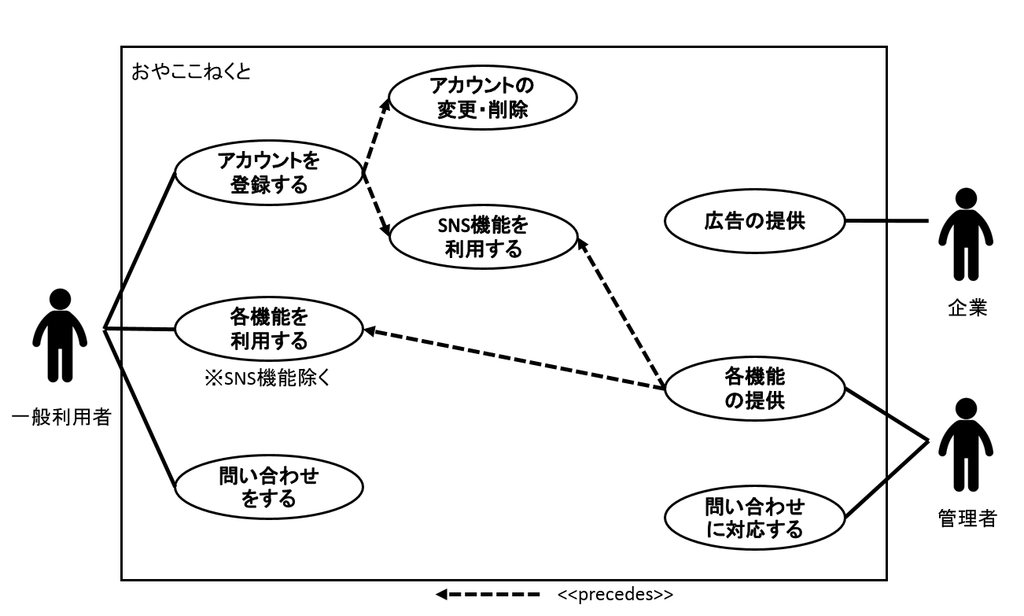
\includegraphics {zentai.png}}
    \caption{システム全体のユースケース図}
    \label{全体}
  \end{center}
\end{figure}

\begin{figure}[H]
  \begin{center}
     \resizebox{8cm}{!}{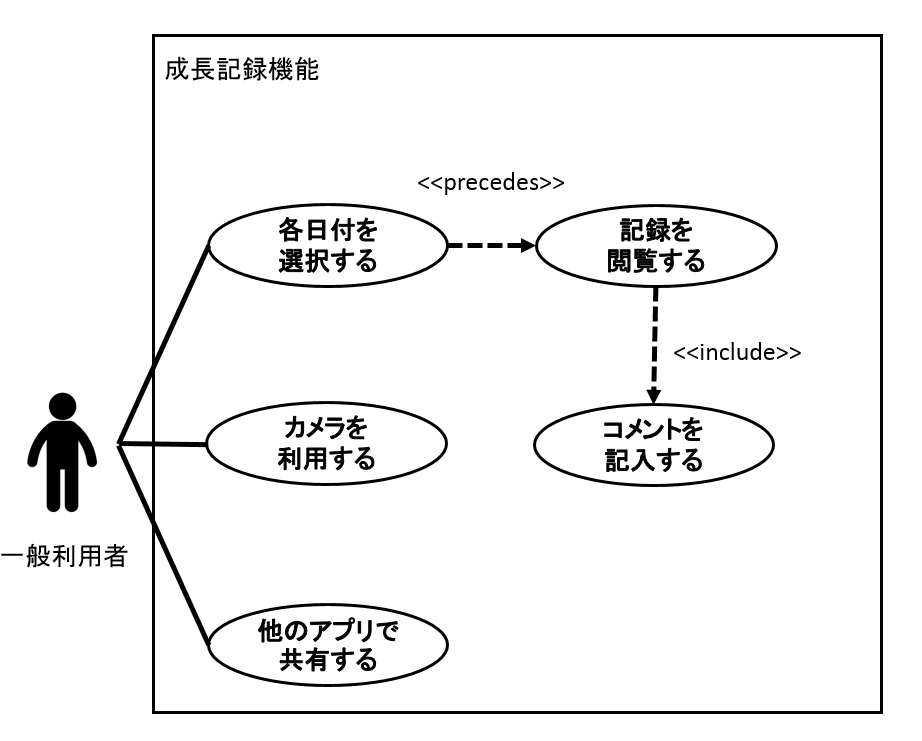
\includegraphics{seithou.png}}
    \caption{成長記録機能のユースケース図}
    \label{成長記録}
  \end{center}
\end{figure}

\begin{figure}[H]
  \begin{center}
     \resizebox{8cm}{!}{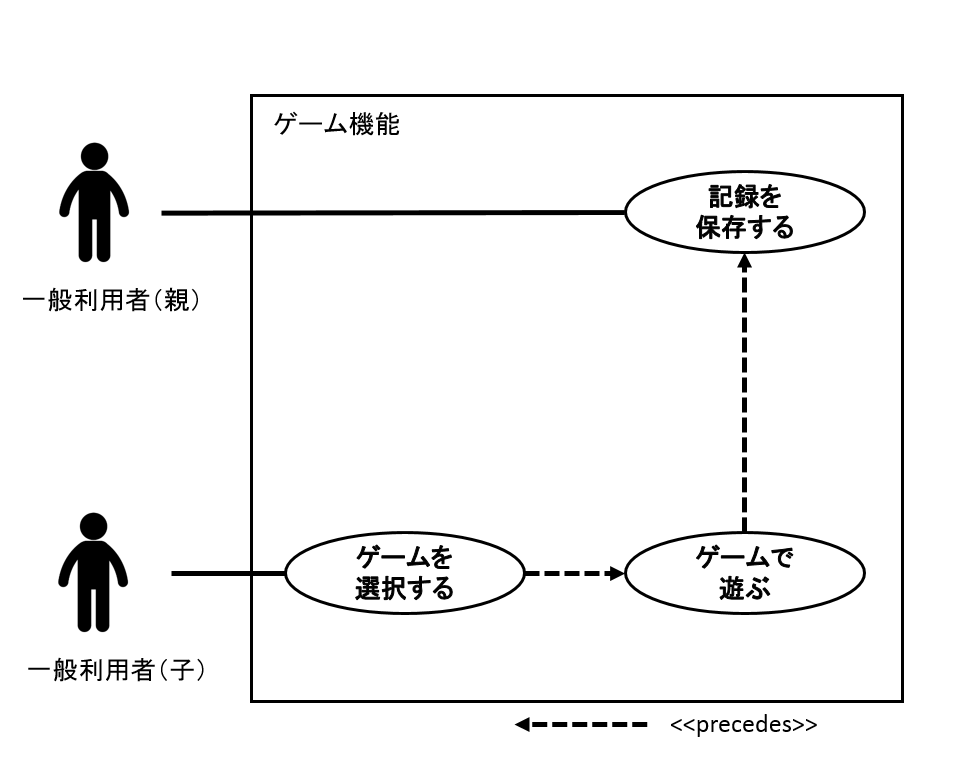
\includegraphics{ugame.png}}
    \caption{ゲーム機能のユースケース図}
    \label{ゲーム}
  \end{center}
\end{figure}

\begin{figure}[H]
  \begin{center}
     \resizebox{8cm}{!}{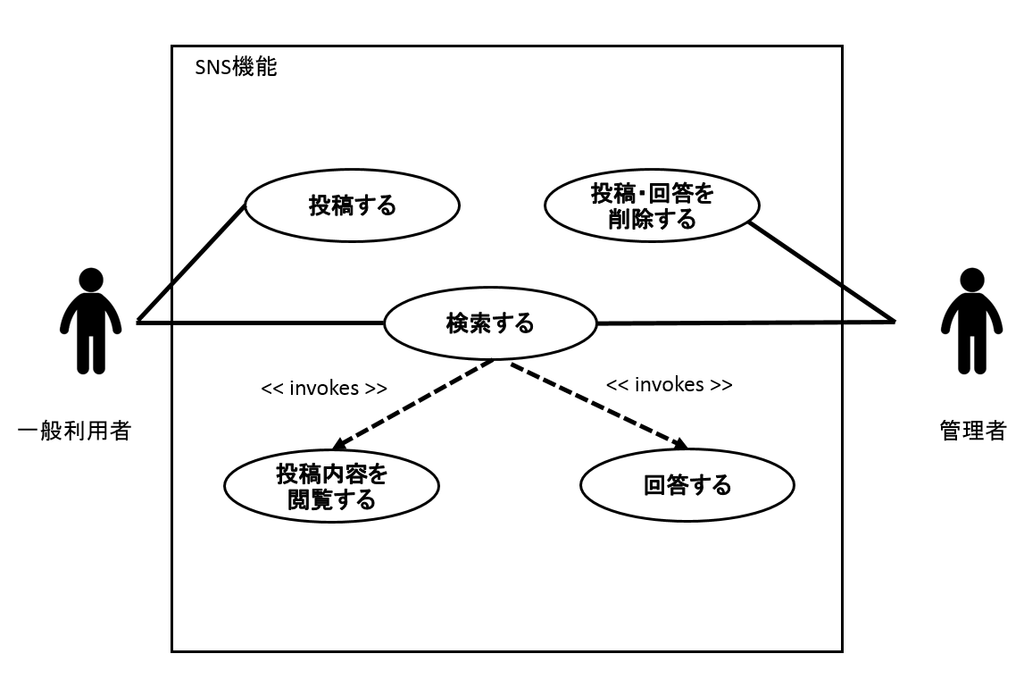
\includegraphics{sns.png}}
    \caption{子育て窓口機能のユースケース図}
    \label{SNS}
  \end{center}
\end{figure}

\end{document}
